\documentclass [a4paper,12pt,oneside,final]{article}
\usepackage[left=15mm,top=15mm,right=15mm,bottom=20mm]{geometry}
\usepackage{tikz}
\usepackage{float}
\usetikzlibrary{arrows,positioning,shapes.geometric}

\title{%
Redes Neuronales \\
Análisis del modelo de Lotka Volterra \\*[23pt]
Trabajo Práctico 1 \\
}
\date{2020}
\author{Igor Andruskiewitsch}

\begin{document}
    \maketitle

\section{Introducción}

\subsection{Modelo Lotka-Volterra}

Este trabajo está orientado a comprender el {\bf Modelo de predadores y presas de Lotka-Volterra}, descrito como el sistema de dos ecuaciones diferenciales ordinarias (ODEs):

\[ \dot{C}(t) = \alpha C(t) - \beta C(t) Z(t) \]
\[ \dot{Z}(t) = - \gamma Z(t) + \delta C(t) Z(t) \]

Donde:

\begin{itemize}
    \item {$ C(t) $ modela el número de presas de un ecosistema}
    \item {$ Z(t) $ modela el número de depredadores en el mismo ecosistema}
\end{itemize}

\subsection{Objetivos}

\begin{itemize}
    \item {Comprender las herramientas disponibles para analizar ODEs}
    \item {Utilizar estas herramientas para comprender el comportamiento del modelo de Lotka-Volterra y extraer conclusiones}
\end{itemize}

\subsection{Parámetros}

Los parámetros $\alpha$, $\beta$, $\gamma$ y $\delta$ del modelo de Lotka-Volterra representan:

\begin{itemize}
    \item{$\alpha$: Tasa de natalidad de las presas}
    \item{$\beta$: Tasa de mortalidad de las presas}
    \item{$\gamma$: Tasa de natalidad de los depredadores}
    \item{$\delta$: Tasa de mortalidad de los depredadores}
\end{itemize}

Se considerarán los siguientes valores para los parámetros:
\[ \alpha = 0.1 \qquad \beta = 0.02 \qquad \gamma = 0.3 \qquad \delta = 0.01 \]


\section{Diagrama de flujo}

Para comprender el comportamiento del modelo, debemos comenzar por entender su flujo, es decir, la tendencia de crecimiento/decrecimiento de nuestras presas/depredadores y su relación.
Podemos considerar 4 diferentes estados:

\begin{center}
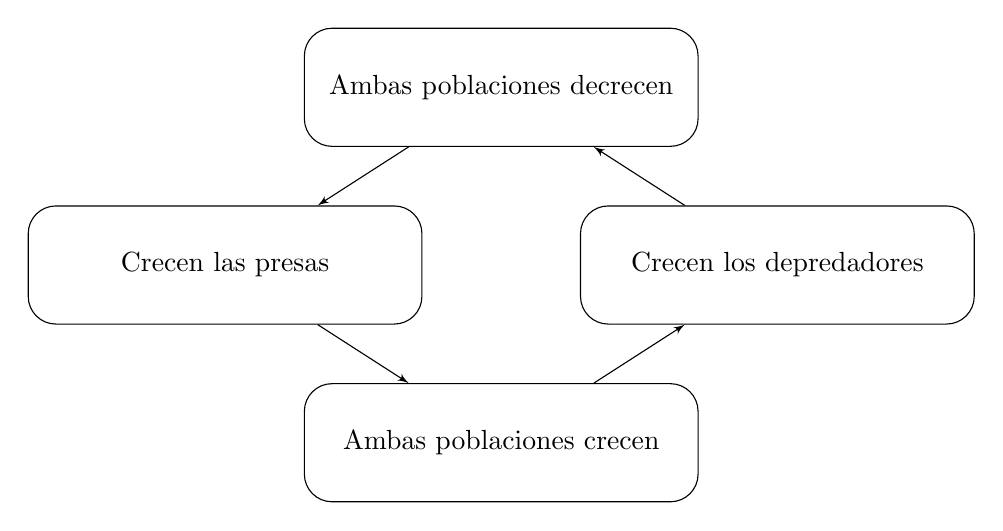
\begin{tikzpicture}[>=latex' ]
        \tikzset{block/.style={draw,
                shape=rectangle,
                align=center,
                rounded corners=1em,
                minimum width=5cm,
                minimum height=1.5cm
            },
        }
        \node [block] (decrecen)
            {Ambas poblaciones decrecen};
        \node [block, below =3cm of decrecen] (crecen)
            {Ambas poblaciones crecen};
        \node [block, below left =1.5cm and =3cm of decrecen] (crecen_p)
            {Crecen las presas};
        \node [block, below right =1.5cm and =-3cm of decrecen] (crecen_d)
            {Crecen los depredadores};
%% paths
\path[draw,->] 
    (decrecen) edge (crecen_p)
    (crecen) edge (crecen_d)
    (crecen_p) edge (crecen)
    (crecen_d) edge (decrecen)
;
\end{tikzpicture}
\end{center}

Podemos ver en este diagrama que aparentemente no hay equilibro entre ambas poblaciones, por el contrario, parece que podrían caer en un ciclo.

\section{Diagrama de fase}

El diagrama de fase es una herramienta que nos permite entender la relación entre las poblaciones. Vamos a aproximar las tasas de crecimiento de ambas poblaciones utilizando el algoritmo de Runge Kutta de 4to orden (RK4), utilizando distintos puntos iniciales (generados al azar utilizando la distribución uniforme) para observar las tendencias en la relación. A su vez, vamos a mostrar en conjunto los vectores que indican la dirección:

\begin{figure}[H]
    \centering
    \includegraphics[width=15cm,keepaspectratio]{./diagramas/fases.png}
    \caption{Diagrama de Fase}\label{fig:fase}
\end{figure}

Podemos observar en el grafico \ref{fig:fase} que todos siguen la dirección marcada por el campo de vectores y que en ninguno de los casos las poblaciones se estabilizan, por el contrario, siguen un ciclo.


\section{Evolución a través del tiempo}

Buscamos una solución aproximada (nuevamente usando RK4) utilizando un punto inicial $(40, 9)$ y valores de $t$ en $(0, 200)$. El grafico resultante es:

\begin{figure}[H]
    \centering
    \includegraphics[width=15cm,keepaspectratio]{./diagramas/evolucion.png}
    \caption{Evolución}\label{fig:time}
\end{figure}

Podemos observar en la figura \ref{fig:time} que el crecimiento de ambas poblaciones se corresponde con el descripto en el diagrama de flujo antes mencionado. Además, el modelo no parece estabilizarse en ningún punto, si no que varía constantemente a través del tiempo.

\section{Conclusión}

Se utilizó el método de Runge-Kutta de 4to Orden para aproximar el comportamiento del modelo. Se vió que para los parámetros elegidos el modelo parece no ser estable, es decir que parece no tener puntos para los cuales los valores de las poblaciones se estabilizan. Por otro lado, también se logró comprender distintas herramientas disponibles a la hora de analizar modelos descritos como ODEs como el campo de vectores y una aproximación a través del tiempo.

\end{document}
